\section{Các yêu cầu hệ thống}

\subsection{User Requirements}

\subsubsection{Module 1 – Nhận và hiển thị dữ liệu từ thiết bị}

\textbf{Mục tiêu:} Thu thập dữ liệu cảm biến và hiển thị theo thời gian thực.

\begin{itemize}
    \item (FR1) Hệ thống phải nhận dữ liệu từ các cảm biến nhiệt độ, độ ẩm, ánh sáng, chuyển động và các loại cảm biến mở rộng được định nghĩa trong backend.
    
    \item (FR2) Dashboard Web phải cập nhật dữ liệu mới thông qua API tổng hợp và kênh realtime Server-Sent Events.
    
    \item (FR3) Hệ thống phải hiển thị trạng thái hiện tại của các thiết bị theo capability như \texttt{POWER}, \texttt{SPEED}, \texttt{BRIGHTNESS}, \texttt{MODE}.
    
    \item (FR4) Người dùng phải xem được biểu đồ lịch sử dữ liệu cảm biến theo khoảng thời gian được hỗ trợ trên giao diện History.
    
    \item (FR5) Hệ thống phải lưu trữ dữ liệu cảm biến vào cơ sở dữ liệu để phục vụ việc truy xuất và phân tích sau này.
    
    \item (FR6) Nếu thiết bị không gửi dữ liệu trong khoảng thời gian cấu hình, hệ thống phải cập nhật trạng thái offline và tạo cảnh báo phù hợp.
\end{itemize}

\subsubsection{Module 2 – Kiểm tra dữ liệu vượt ngưỡng}

\textbf{Mục tiêu:} Phát hiện các điều kiện bất thường và tạo cảnh báo.

\begin{itemize}
    \item (FR7) Quản trị viên phải có khả năng cấu hình các ngưỡng an toàn như: nhiệt độ cao/thấp, ánh sáng cao/thấp và nhiệt độ nguy hiểm.
    
    \item (FR8) Nếu nhiệt độ vượt ngưỡng cao trong khoảng thời gian cấu hình (ví dụ 2 phút), hệ thống phải tạo cảnh báo.
    
    \item (FR9) Nếu ánh sáng thấp hơn hoặc cao hơn mức cấu hình, hệ thống phải kích hoạt hành động tự động tương ứng.
    
    \item (FR10) Hệ thống phải áp dụng cơ chế hysteresis để tránh việc thiết bị bật/tắt liên tục khi giá trị cảm biến dao động quanh ngưỡng.
    
    \item (FR11) Khi giá trị vượt ngưỡng nguy hiểm (ví dụ $T_{critical}$), hệ thống phải hiển thị cảnh báo trên dashboard, hỗ trợ thông báo qua kênh được cấu hình và ghi log sự kiện.
    
    \item (FR12) Nếu phát hiện dữ liệu cảm biến không hợp lệ hoặc vượt ngoài miền cho phép, hệ thống phải chuyển thiết bị về trạng thái an toàn và ghi nhận lỗi.
    
    \item (FR13) Mỗi cảnh báo phải có ba trạng thái: \textit{Active}, \textit{Acknowledged} và \textit{Resolved}.
\end{itemize}

\subsubsection{Module 3 – Điều khiển thiết bị}

\textbf{Mục tiêu:} Cho phép người dùng điều khiển thiết bị theo cách thủ công hoặc tự động.

\begin{itemize}
    \item (FR14) Người dùng phải có khả năng điều khiển thiết bị từ dashboard Web và theo dõi trạng thái lệnh.
    
    \item (FR15) Thiết bị/simulator hỗ trợ nhập mật khẩu bảo mật qua luồng hồng ngoại; khi nhập sai quá số lần cấu hình, hệ thống tạo cảnh báo và ghi log sự kiện.
    
    \item (FR16) Khi người dùng điều khiển thủ công trong chế độ tự động, hệ thống phải chuyển sang chế độ MANUAL, giữ trạng thái thiết bị trong thời gian $T_{hold}$ và sau đó quay lại chế độ trước đó.
    
    \item (FR17) Trong chế độ AUTO, hệ thống phải tự động điều khiển quạt theo nhiệt độ và đèn theo mức ánh sáng.
    
    \item (FR18) Trong chế độ SLEEP, hệ thống phải ưu tiên tiết kiệm điện và giảm mức hoạt động của thiết bị.
    
    \item (FR19) Trong chế độ AWAY, hệ thống phải tắt các thiết bị không cần thiết và chỉ kích hoạt khi vượt ngưỡng an toàn.
    
    \item (FR20) Quản trị viên phải có khả năng cấu hình lịch tự động chuyển đổi giữa các chế độ AUTO, SLEEP và AWAY theo khung giờ.
\end{itemize}

\subsubsection{Module 4 – Ghi nhận hoạt động (Logging và Audit)}

\textbf{Mục tiêu:} Theo dõi và lưu trữ toàn bộ hoạt động của hệ thống.

\begin{itemize}
    \item (FR21) Mọi hành động bật/tắt thiết bị phải được ghi log bao gồm: người thực hiện, thời điểm và trạng thái trước/sau của thiết bị.
    
    \item (FR22) Mọi cảnh báo phải được lưu lại với các thông tin: thời điểm kích hoạt, thời điểm xác nhận và thời điểm kết thúc.
    
    \item (FR23) Mọi thay đổi cấu hình hệ thống như thay đổi ngưỡng, lịch hoạt động hoặc chế độ mặc định phải được ghi log đầy đủ.
    
    \item (FR24) Quản trị viên phải có khả năng truy xuất và lọc lịch sử hoạt động theo thời gian, loại sự kiện và người thực hiện.
\end{itemize}

\subsubsection{Module 5 – Ứng dụng Web}

\textbf{Mục tiêu:} Cung cấp giao diện sử dụng và phân quyền truy cập.

\begin{itemize}
    \item (FR25) Hệ thống phải yêu cầu người dùng đăng nhập bằng tài khoản cục bộ hoặc Google OAuth để truy cập các chức năng được bảo vệ.
    
    \item (FR26) Hệ thống phải hỗ trợ phân quyền người dùng gồm:
    \begin{itemize}
        \item \texttt{ADMIN}/\texttt{SUPER\_ADMIN}: quản lý người dùng, cấu hình hệ thống và xem audit log.
        \item Người dùng trong home: xem dữ liệu, điều khiển thiết bị và thao tác trong phạm vi quyền home.
        \item Vai trò home như \texttt{OWNER}, \texttt{CO\_OWNER}, \texttt{RESIDENT}, \texttt{TECHNICIAN}, \texttt{VIEWER} quyết định quyền ở cấp nhà.
    \end{itemize}
    
    \item (FR27) Dashboard tổng quan phải hiển thị dữ liệu realtime, trạng thái thiết bị và các cảnh báo hiện tại.
    
    \item (FR28) Quản trị viên phải có khả năng cấu hình ngưỡng và lịch hoạt động trực tiếp từ giao diện hệ thống.
    
    \item (FR29) Người dùng phải xem được cảnh báo mới trên dashboard; các kênh email, Telegram phụ thuộc cấu hình triển khai.
\end{itemize}

\subsection{Yêu cầu chức năng}
Danh sách các actor:
\begin{itemize}
    \item User (Chủ nhà)
    \item Admin (Quản trị hệ thống)
    \item Installer (Bên lắp đặt)
    \item IoT Device (Thiết bị cảm biến \& điều khiển)
    \item System (Hệ thống tự động)

\end{itemize}
Để hiểu rõ thêm về yêu cầu chức năng của hệ thống nhóm tác giả đã mô hình hóa bằng các sơ đồ use-case sau:
\\

% UC1
\begin{table}[H]
\centering
\captionsetup{justification=centering}
\caption*{\textbf{USE CASE 1: ĐĂNG NHẬP HỆ THỐNG}}
\renewcommand{\arraystretch}{1.3}
\begin{tabular}{|p{4cm}|p{11cm}|}
\hline
\textbf{Usecase name} & Đăng nhập hệ thống \\
\hline
\textbf{Description} & Người dùng đăng nhập vào hệ thống để truy cập chức năng theo role. \\
\hline
\textbf{Actors} & User / Admin / Installer \\
\hline
\textbf{Preconditions} & Tài khoản hợp lệ tồn tại trong hệ thống. \\
\hline
\textbf{Trigger} & Người dùng nhập username và password. \\
\hline
\multirow{2}{*}{\textbf{Post-conditions}} & 
Success: Tạo session/token và chuyển đến dashboard.\\ &
Failure: Không tạo session. \\
\hline
\textbf{Main flow} & 
1. Nhập thông tin đăng nhập.\\ &
2. Hệ thống xác thực.\\ &
3. Xác định role.\\ &
4. Chuyển hướng dashboard. \\
\hline
\textbf{Alternative flow} & Sai thông tin → Thông báo lỗi. \\
\hline
\textbf{Exceptions} & Lỗi server hoặc database. \\
\hline
\end{tabular}
\end{table}

% UC2
\begin{table}[H]
\centering
\captionsetup{justification=centering}
\caption*{\textbf{USE CASE 2: GỬI DỮ LIỆU CẢM BIẾN}}
\renewcommand{\arraystretch}{1.3}
\begin{tabular}{|p{4cm}|p{11cm}|}
\hline
Usecase name & Gửi dữ liệu cảm biến \\
\hline
Description & Thiết bị gửi dữ liệu định kỳ về server. \\
\hline
Actors & IoT Device \\
\hline
Preconditions & Thiết bị đang hoạt động và có kết nối mạng. \\
\hline
Trigger & Đến chu kỳ gửi dữ liệu. \\
\hline
Post-conditions & Dữ liệu được lưu vào database. \\
\hline
Main flow & 
1. Thu thập dữ liệu.\\ &
2. Gửi lên server.\\ & 
3. Server kiểm tra hợp lệ.\\ &
4. Lưu database. \\
\hline
Alternative flow & Dữ liệu không hợp lệ → Bỏ qua và ghi log. \\
\hline
Exceptions & Mất kết nối mạng. \\
\hline
\end{tabular}
\end{table}
% UC3
\begin{table}[H]
\centering
\captionsetup{justification=centering}
\caption*{\textbf{USE CASE 3: XEM DỮ LIỆU REALTIME}}
\renewcommand{\arraystretch}{1.3}
\begin{tabular}{|p{4cm}|p{11cm}|}
\hline
Usecase name & Xem dữ liệu realtime \\
\hline
Description & Người dùng xem dữ liệu cập nhật theo thời gian thực. \\
\hline
Actors & User \\
\hline
Preconditions & Đã đăng nhập thành công. \\
\hline
Trigger & Mở dashboard. \\
\hline
Post-conditions & Dữ liệu hiển thị $\le$ 2 giây sau khi cập nhật. \\
\hline
Main flow & 
1. Truy cập dashboard.\\ &
2. Hệ thống lấy dữ liệu mới nhất.\\ &
3. Hiển thị lên giao diện. \\
\hline
Alternative flow & Không có dữ liệu → Hiển thị trạng thái chờ. \\
\hline
Exceptions & Lỗi truy vấn database. \\
\hline
\end{tabular}
\end{table}
% UC4
\begin{table}[H]
\centering
\caption*{\textbf{USE CASE 4: XEM BIỂU ĐỒ LỊCH SỬ}}
\renewcommand{\arraystretch}{1.3}
\begin{tabular}{|p{4cm}|p{11cm}|}
\hline
Usecase name & Xem biểu đồ lịch sử \\
\hline
Description & Xem dữ liệu theo 1h, 24h, 7 ngày. \\
\hline
Actors & User \\
\hline
Preconditions & Có dữ liệu lưu trữ. \\
\hline
Trigger & Chọn khoảng thời gian. \\
\hline
Post-conditions & Hiển thị biểu đồ tương ứng. \\
\hline
Main flow & 
1. Chọn loại dữ liệu.\\ &
2. Chọn mốc thời gian.\\ &
3. Hệ thống truy vấn.\\ &
4. Hiển thị biểu đồ. \\
\hline
Alternative flow & Không có dữ liệu → Thông báo. \\
\hline
Exceptions & Lỗi truy vấn. \\
\hline
\end{tabular}
\end{table}
% UC5
\begin{table}[H]
\centering
\caption*{\textbf{USE CASE 5: XEM TRẠNG THÁI THIẾT BỊ}}
\renewcommand{\arraystretch}{1.3}
\begin{tabular}{|p{4cm}|p{11cm}|}
\hline
Usecase name & Xem trạng thái thiết bị \\
\hline
Description & Hiển thị ON/OFF hoặc Offline. \\
\hline
Actors & User \\
\hline
Preconditions & Đã đăng nhập. \\
\hline
Trigger & Mở dashboard. \\
\hline
Post-conditions & Trạng thái hiển thị chính xác. \\
\hline
Main flow & 
1. Hệ thống lấy trạng thái thiết bị.\\ &
2. Hiển thị ON/OFF. \\
\hline
Alternative flow & Không phản hồi → Hiển thị Offline. \\
\hline
Exceptions & Mất kết nối thiết bị. \\
\hline
\end{tabular}
\end{table}
% UC6
\begin{table}[H]
\centering
\caption*{\textbf{USE CASE 6: CẤU HÌNH NGƯỠNG CẢNH BÁO}}
\renewcommand{\arraystretch}{1.3}
\begin{tabular}{|p{4cm}|p{11cm}|}
\hline
Usecase name & Cấu hình ngưỡng cảnh báo \\
\hline
Description & Admin thiết lập giá trị ngưỡng high/low/critical cho cảm biến. \\
\hline
Actors & Admin \\
\hline
Preconditions & Admin đã đăng nhập. \\
\hline
Trigger & Admin truy cập trang cấu hình. \\
\hline
Post-conditions & Ngưỡng mới được lưu vào hệ thống. \\
\hline
Main flow &
1. Mở trang cấu hình.\\ & 
2. Nhập giá trị ngưỡng.\\ &
3. Nhấn lưu.\\ &
4. Hệ thống kiểm tra hợp lệ.\\ &
5. Lưu vào database. \\
\hline
Alternative flow & Giá trị không hợp lệ → Thông báo lỗi. \\
\hline
Exceptions & Lỗi lưu database. \\
\hline
\end{tabular}
\end{table}
% UC7
\begin{table}[H]
\centering
\caption*{\textbf{USE CASE 7: PHÁT HIỆN VƯỢT NGƯỠNG}}
\renewcommand{\arraystretch}{1.3}
\begin{tabular}{|p{4cm}|p{11cm}|}
\hline
Usecase name & Phát hiện vượt ngưỡng \\
\hline
Description & Hệ thống kiểm tra dữ liệu và phát hiện giá trị bất thường. \\
\hline
Actors & System \\
\hline
Preconditions & Có dữ liệu cảm biến mới. \\
\hline
Trigger & Nhận dữ liệu từ thiết bị. \\
\hline
Post-conditions & Tạo cảnh báo trạng thái Active nếu vượt ngưỡng. \\
\hline
Main flow &
1. Nhận dữ liệu mới.\\ &
2. So sánh với ngưỡng cấu hình.\\ &
3. Kiểm tra thời gian duy trì vượt ngưỡng.\\ &
4. Tạo cảnh báo. \\
\hline
Alternative flow & Không vượt ngưỡng → Không tạo cảnh báo. \\
\hline
Exceptions & Lỗi xử lý dữ liệu. \\
\hline
\end{tabular}
\end{table}
% UC8
\begin{table}[H]
\centering
\caption*{\textbf{USE CASE 8: GỬI CẢNH BÁO}}
\renewcommand{\arraystretch}{1.3}
\begin{tabular}{|p{4cm}|p{11cm}|}
\hline
Usecase name & Gửi cảnh báo \\
\hline
Description & Hệ thống gửi thông báo khi có cảnh báo mới. \\
\hline
Actors & System \\
\hline
Preconditions & Cảnh báo đã được tạo. \\
\hline
Trigger & Trạng thái cảnh báo = Active. \\
\hline
Post-conditions & Người dùng và installer nhận thông báo. \\
\hline
Main flow &
1. Hiển thị cảnh báo trên dashboard.\\ &
2. Gửi notification/email.\\ &
3. Ghi log sự kiện. \\
\hline
Alternative flow & Gửi email thất bại → Ghi log lỗi. \\
\hline
Exceptions & Lỗi dịch vụ gửi email. \\
\hline
\end{tabular}
\end{table}
% UC9
\begin{table}[H]
\centering
\caption*{\textbf{USE CASE 9: XÁC NHẬN CẢNH BÁO}}
\renewcommand{\arraystretch}{1.3}
\begin{tabular}{|p{4cm}|p{11cm}|}
\hline
Usecase name & Xác nhận cảnh báo \\
\hline
Description & User/Admin xác nhận cảnh báo đang Active và Installer xác nhận Resolved sau khi giải quyết. \\
\hline
Actors & User / Admin / Installer \\
\hline
Preconditions & Có cảnh báo trạng thái Active. \\
\hline
Trigger & Admin hoặc User nhấn nút Acknowledge. Installer nhấn nút Resolved  \\
\hline
Post-conditions & Trạng thái chuyển sang Acknowledged khi xác nhận lỗi và chuyển sang Resolved khi đã sửa. \\
\hline
Main flow &
1. Chọn cảnh báo.\\ &
2. Nhấn Acknowledge/Resolved.\\ &
3. Hệ thống cập nhật trạng thái.\\ &
4. Ghi log. \\
\hline
Alternative flow & Cảnh báo đã được xử lý trước đó. \\
\hline
Exceptions & Lỗi cập nhật database. \\
\hline
\end{tabular}
\end{table}
% UC10
\begin{table}[H]
\centering
\caption*{\textbf{USE CASE 10: ĐIỀU KHIỂN THỦ CÔNG}}
\renewcommand{\arraystretch}{1.3}
\begin{tabular}{|p{4cm}|p{11cm}|}
\hline
Usecase name & Điều khiển thiết bị thủ công \\
\hline
Description & User bật/tắt thiết bị từ dashboard. \\
\hline
Actors & User \\
\hline
Preconditions & Thiết bị đang online. \\
\hline
Trigger & Nhấn nút ON/OFF. \\
\hline
Post-conditions & Thiết bị đổi trạng thái thành công. \\
\hline
Main flow &
1. User chọn thiết bị.\\ &
2. Nhấn ON/OFF.\\ &
3. Hệ thống gửi lệnh.\\ &
4. Thiết bị phản hồi.\\ &
5. Cập nhật giao diện. \\
\hline
Alternative flow & Thiết bị không phản hồi → Thông báo lỗi. \\
\hline
Exceptions & Mất kết nối HTTP/API hoặc thiết bị. \\
\hline
\end{tabular}
\end{table}
% UC11
\begin{table}[H]
\centering
\caption*{\textbf{USE CASE 11: XÁC THỰC MẬT KHẨU NHÀ}}
\renewcommand{\arraystretch}{1.3}
\begin{tabular}{|p{4cm}|p{11cm}|}
\hline
Usecase name & Xác thực mật khẩu nhà \\
\hline
Description & Kiểm tra quyền truy cập qua mật khẩu tại thiết bị. \\
\hline
Actors & User \\
\hline
Preconditions & Thiết bị hoạt động. \\
\hline
Trigger & Người dùng nhập mật khẩu. \\
\hline
Post-conditions & Đăng nhập thành công. \\
\hline
Main flow &
1. Người dùng nhập mật khẩu\\ &
2. Hệ thống kiểm tra mật khẩu chính xác. \\ &
3. Nếu đúng, cho phép truy cập hệ thống\\ 
\hline
Alternative flow & Nhập mật khẩu sai → Hệ thống đếm số lần nhập sai → Nếu quá 3 lần sai, hệ thống báo động, gửi cảnh báo cho chủ nhà, ghi log cho sự kiện \\
\hline
Exceptions & Mất kết nối hệ thống hoặc thiết bị.  \\
\hline
\end{tabular}
\end{table}
% UC12
\begin{table}[H]
\centering
\caption*{\textbf{USE CASE 12: MANUAL OVERRIDE}}
\renewcommand{\arraystretch}{1.3}
\begin{tabular}{|p{4cm}|p{11cm}|}
\hline
Usecase name & Manual Override \\
\hline
Description & Chuyển sang chế độ MANUAL khi user điều khiển trong AUTO. \\
\hline
Actors & User \\
\hline
Preconditions & Hệ thống đang ở chế độ AUTO. \\
\hline
Trigger & User thực hiện điều khiển thủ công. \\
\hline
Post-conditions & Sau Thold phút quay lại AUTO. \\
\hline
Main flow &
1. Phát hiện lệnh thủ công.\\ &
2. Chuyển sang MANUAL.\\ &
3. Giữ trạng thái Thold phút.\\ &
4. Tự động quay lại AUTO. \\
\hline
Alternative flow & User tiếp tục thao tác → Reset thời gian Thold. \\
\hline
Exceptions & Lỗi timer hệ thống. \\
\hline
\end{tabular}
\end{table}
% UC13
\begin{table}[H]
\centering
\caption*{\textbf{USE CASE 13: CHUYỂN CHẾ ĐỘ HOẠT ĐỘNG}}
\renewcommand{\arraystretch}{1.3}
\begin{tabular}{|p{4cm}|p{11cm}|}
\hline
Usecase name & Chuyển chế độ hoạt động \\
\hline
Description & Người dùng chuyển đổi giữa AUTO, SLEEP, AWAY. \\
\hline
Actors & User \\
\hline
Preconditions & Đã đăng nhập hệ thống. \\
\hline
Trigger & Chọn chế độ trên dashboard. \\
\hline
Post-conditions & Hệ thống áp dụng rule tương ứng với mode mới. \\
\hline
Main flow &
1. Người dùng chọn mode.\\ &
2. Hệ thống xác nhận yêu cầu.\\ &
3. Cập nhật mode hiện tại.\\ &
4. Áp dụng rule điều khiển thiết bị. \\
\hline
Alternative flow & Mode đã được chọn trước đó → Không thay đổi. \\
\hline
Exceptions & Lỗi cập nhật database. \\
\hline
\end{tabular}
\end{table}
% UC14
\begin{table}[H]
\centering
\caption*{\textbf{USE CASE 14: LẬP LỊCH CHUYỂN CHẾ ĐỘ}}
\renewcommand{\arraystretch}{1.3}
\begin{tabular}{|p{4cm}|p{11cm}|}
\hline
Usecase name & Lập lịch chuyển chế độ \\
\hline
Description & Admin cấu hình lịch tự động chuyển mode theo thời gian. \\
\hline
Actors & Admin \\
\hline
Preconditions & Admin đã đăng nhập. \\
\hline
Trigger & Truy cập trang cấu hình lịch. \\
\hline
Post-conditions & Lịch được lưu và tự động thực thi theo thời gian cấu hình. \\
\hline
Main flow &
1. Nhập thời gian bắt đầu/kết thúc.\\ &
2. Chọn mode tương ứng.\\ &
3. Lưu cấu hình.\\ &
4. Hệ thống kích hoạt scheduler. \\
\hline
Alternative flow & Thời gian trùng lặp → Thông báo lỗi. \\
\hline
Exceptions & Lỗi hệ thống scheduler. \\
\hline
\end{tabular}
\end{table}
% UC15
\begin{table}[H]
\centering
\caption*{\textbf{USE CASE 15: GHI LOG ĐIỀU KHIỂN}}
\renewcommand{\arraystretch}{1.3}
\begin{tabular}{|p{4cm}|p{11cm}|}
\hline
Usecase name & Ghi log điều khiển thiết bị \\
\hline
Description & Hệ thống ghi nhận mọi hành động bật/tắt thiết bị. \\
\hline
Actors & System \\
\hline
Preconditions & Có hành động điều khiển thiết bị. \\
\hline
Trigger & User/Admin thực hiện điều khiển. \\
\hline
Post-conditions & Log được lưu vào database. \\
\hline
Main flow &
1. Nhận sự kiện điều khiển.\\ &
2. Ghi user, thời gian, trạng thái trước/sau.\\ &
3. Lưu database. \\
\hline
Alternative flow & Không có thay đổi trạng thái → Không ghi log. \\
\hline
Exceptions & Lỗi ghi database. \\
\hline
\end{tabular}
\end{table}
% UC16
\begin{table}[H]
\centering
\caption*{\textbf{USE CASE 16: GHI LOG CẢNH BÁO}}
\renewcommand{\arraystretch}{1.3}
\begin{tabular}{|p{4cm}|p{11cm}|}
\hline
Usecase name & Ghi log cảnh báo \\
\hline
Description & Lưu lại toàn bộ vòng đời của cảnh báo. \\
\hline
Actors & System \\
\hline
Preconditions & Có cảnh báo được tạo. \\
\hline
Trigger & Trạng thái cảnh báo thay đổi. \\
\hline
Post-conditions & Lưu thời điểm Active/Acknowledge/Resolved. \\
\hline
Main flow &
1. Nhận sự kiện thay đổi trạng thái.\\ &
2. Cập nhật thời điểm tương ứng.\\ &
3. Lưu vào database. \\
\hline
Alternative flow & Không thay đổi trạng thái → Không cập nhật. \\
\hline
Exceptions & Lỗi database. \\
\hline
\end{tabular}
\end{table}
% UC17
\begin{table}[H]
\centering
\caption*{\textbf{USE CASE 17: XEM \& LỌC LOG}}
\renewcommand{\arraystretch}{1.3}
\begin{tabular}{|p{4cm}|p{11cm}|}
\hline
Usecase name & Xem và lọc log hệ thống \\
\hline
Description & Admin xem và lọc log theo tiêu chí. \\
\hline
Actors & Admin \\
\hline
Preconditions & Đã có dữ liệu log. \\
\hline
Trigger & Truy cập trang log. \\
\hline
Post-conditions & Hiển thị danh sách log phù hợp điều kiện lọc. \\
\hline
Main flow &
1. Chọn bộ lọc (thời gian, loại sự kiện, người dùng).\\ &
2. Hệ thống truy vấn database.\\ &
3. Hiển thị kết quả. \\
\hline
Alternative flow & Không có kết quả → Hiển thị rỗng. \\
\hline
Exceptions & Lỗi truy vấn database. \\
\hline
\end{tabular}
\end{table}
% UC18
\begin{table}[H]
\centering
\caption*{\textbf{USE CASE 18: PHÂN QUYỀN HỆ THỐNG}}
\renewcommand{\arraystretch}{1.3}
\begin{tabular}{|p{4cm}|p{11cm}|}
\hline
Usecase name & Phân quyền truy cập \\
\hline
Description & Hệ thống phân quyền theo role (Admin, User, Installer). \\
\hline
Actors & System \\
\hline
Preconditions & Người dùng đã đăng nhập. \\
\hline
Trigger & Sau khi xác thực thành công. \\
\hline
Post-conditions & Người dùng chỉ truy cập chức năng phù hợp role. \\
\hline
Main flow &
1. Xác định role người dùng.\\ &
2. Áp dụng quyền truy cập tương ứng.\\ &
3. Chặn truy cập trái phép. \\
\hline
Alternative flow & Role không hợp lệ → Từ chối truy cập. \\
\hline
Exceptions & Lỗi kiểm tra quyền. \\
\hline
\end{tabular}
\end{table}
% UC19
\begin{table}[H]
\centering
\caption*{\textbf{USE CASE 19: DASHBOARD THEO TỪNG CHỦ NHÀ}}
\renewcommand{\arraystretch}{1.3}
\begin{tabular}{|p{4cm}|p{11cm}|}
\hline
Usecase name & Dashboard riêng theo từng chủ nhà \\
\hline
Description & Mỗi User chỉ xem và điều khiển thiết bị thuộc home của mình. \\
\hline
Actors & User \\
\hline
Preconditions & User đã đăng nhập. \\
\hline
Trigger & Truy cập dashboard. \\
\hline
Post-conditions & Chỉ hiển thị thiết bị thuộc quyền sở hữu. \\
\hline
Main flow &
1. Lấy home\_id của user.\\ &
2. Truy vấn danh sách thiết bị tương ứng.\\ &
3. Hiển thị dashboard cá nhân hóa. \\
\hline
Alternative flow & Không có thiết bị → Hiển thị dashboard trống. \\
\hline
Exceptions & Lỗi truy vấn database. \\
\hline
\end{tabular}
\end{table}

\begin{figure}[H]
    \centering
    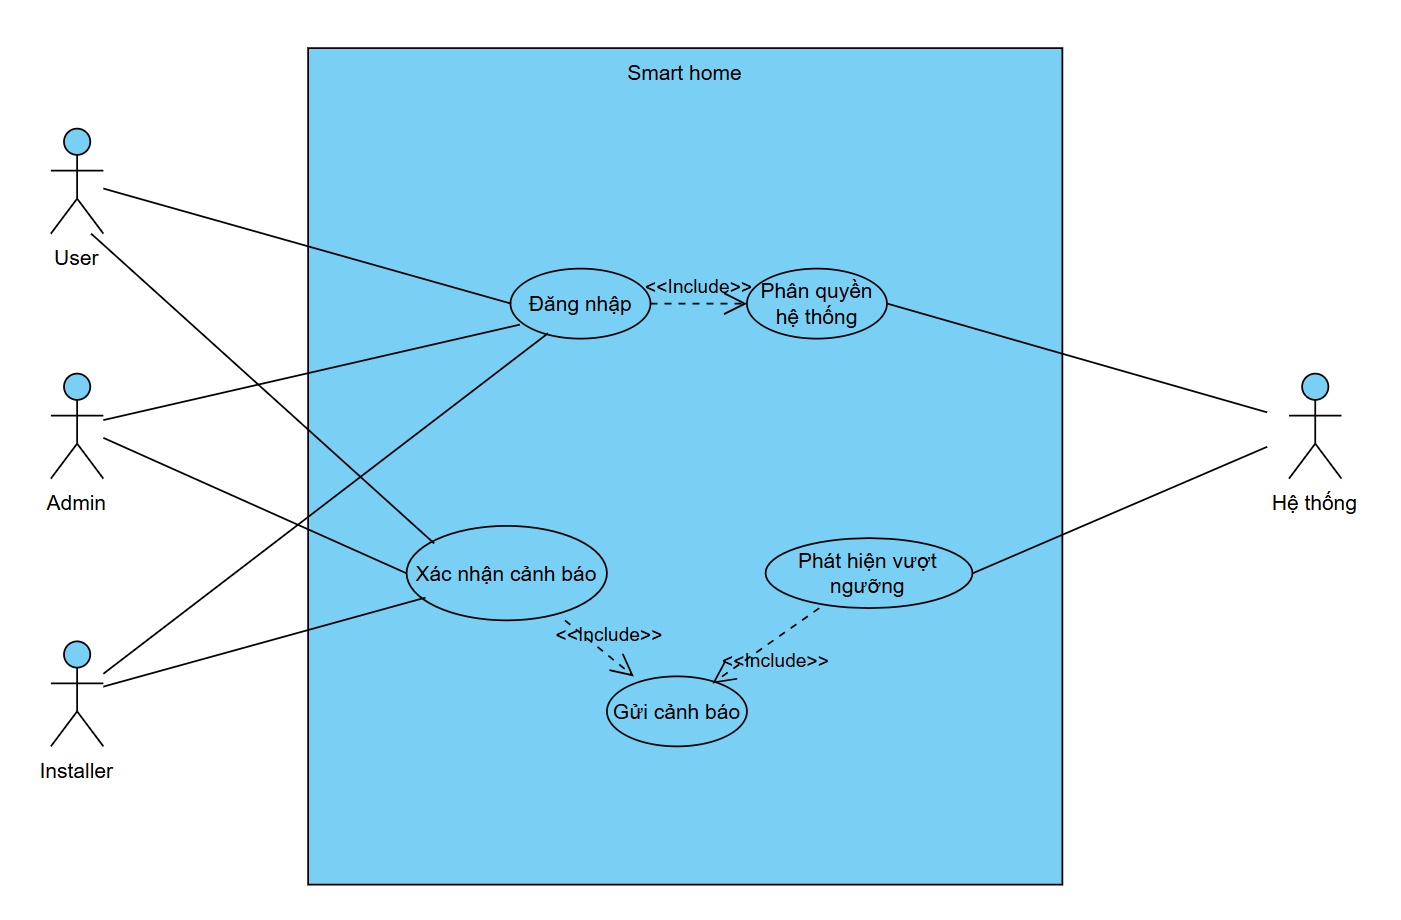
\includegraphics[width=\linewidth,height=0.78\textheight,keepaspectratio]{Images/func-req1.png.png}
    \caption{Biểu đồ use-case 1,7,8,9,18}
\end{figure}

\begin{figure}[H]
    \centering
    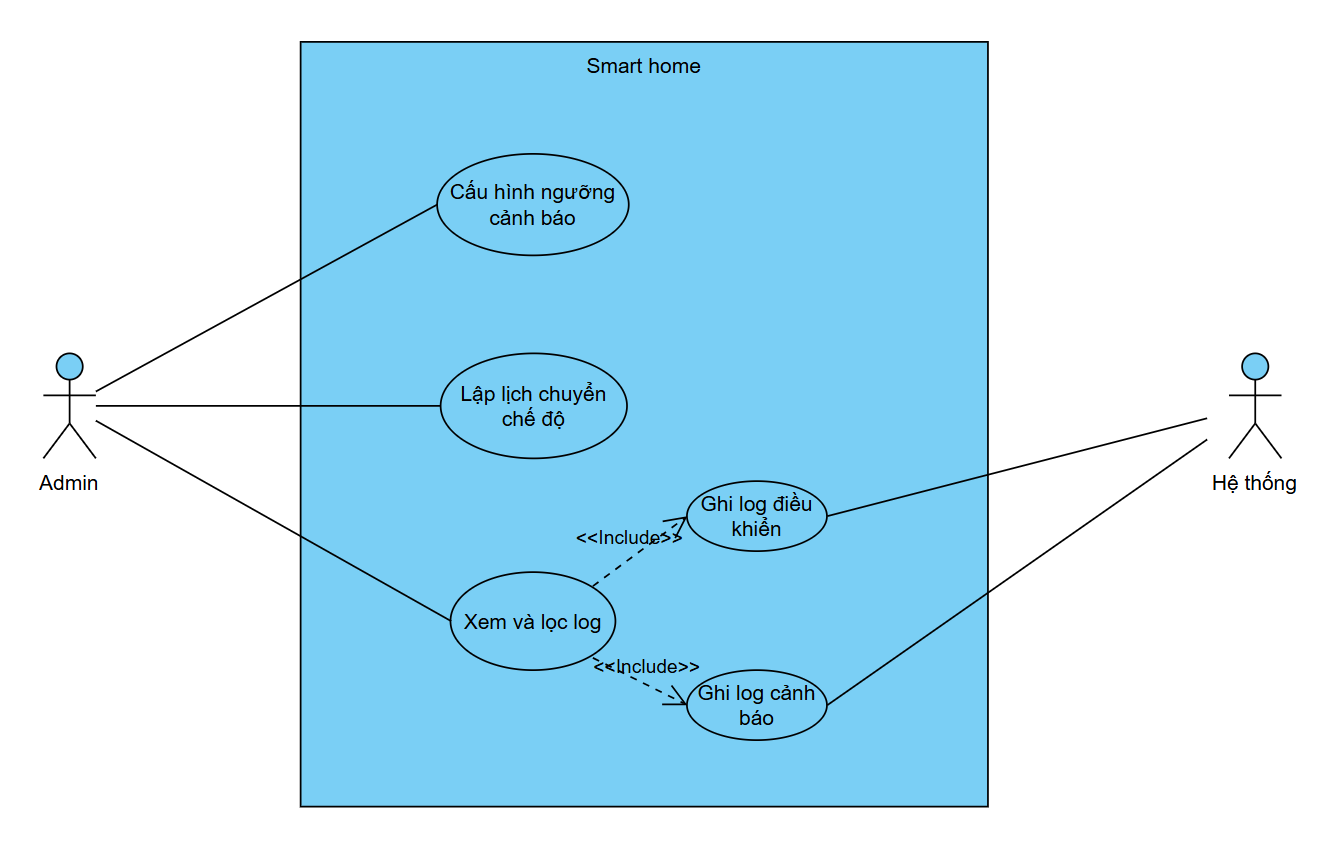
\includegraphics[width=\linewidth,height=0.78\textheight,keepaspectratio]{Images/func-req2.png.png}
    \caption{Biểu đồ use-case 6,14,15,16,17}
\end{figure}

\begin{figure}[H]
    \centering
    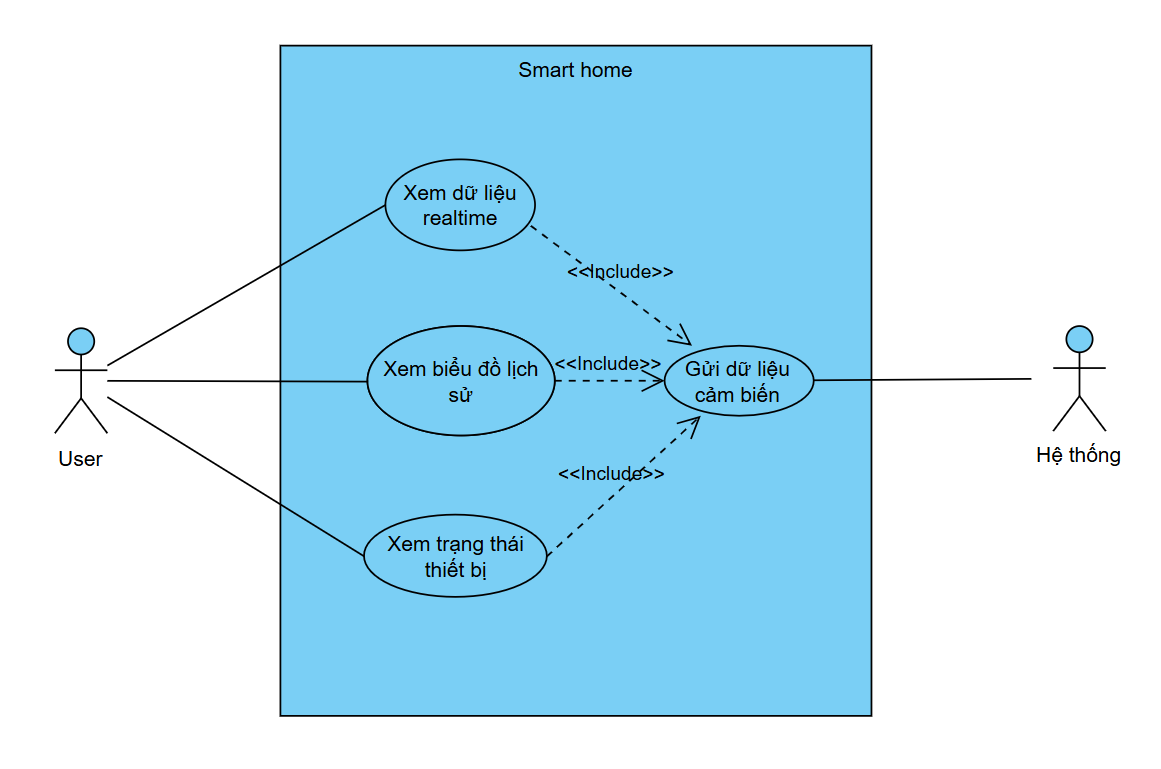
\includegraphics[width=\linewidth,height=0.78\textheight,keepaspectratio]{Images/func-req3.png.png}
    \caption{Biểu đồ use-case 2,3,4,5}
\end{figure}

\begin{figure}[H]
    \centering
    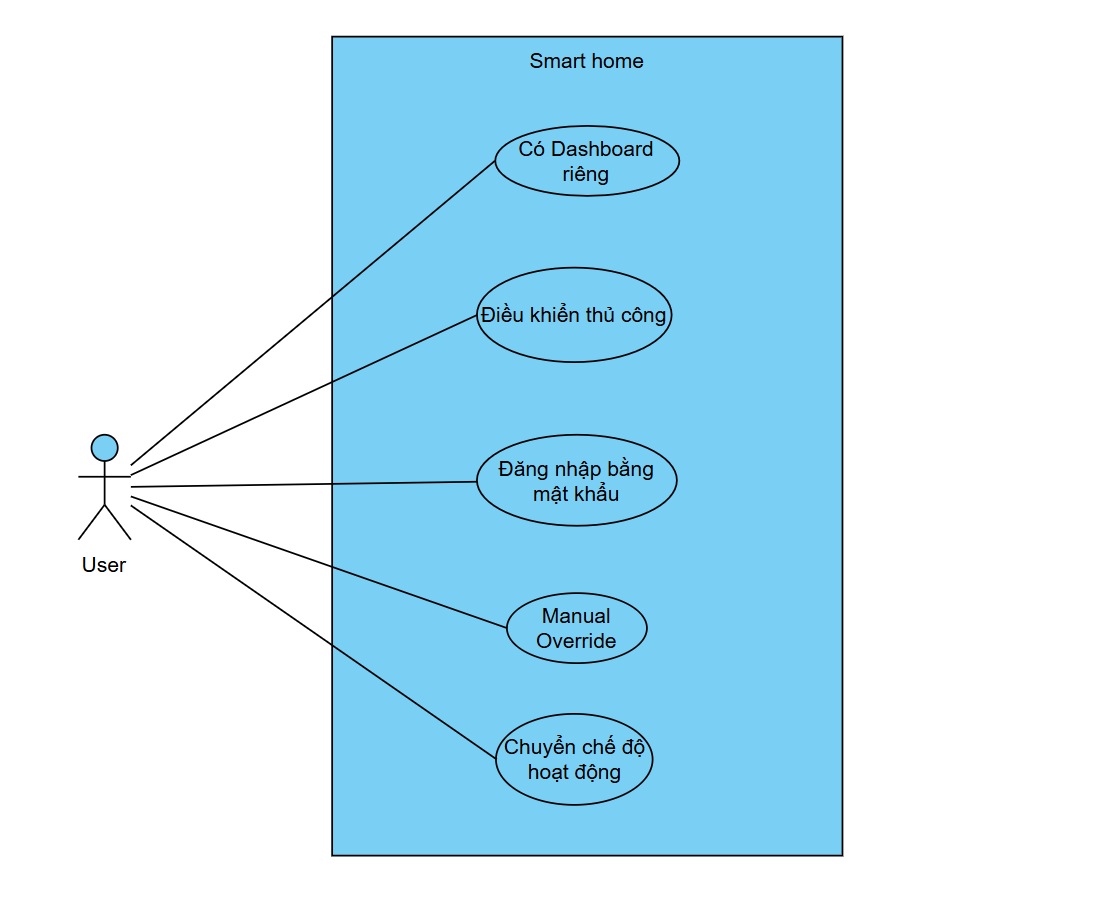
\includegraphics[width=\linewidth,height=0.78\textheight,keepaspectratio]{Images/func-req4.png.png}
    \caption{Biểu đồ use-case 10,11,12,13}
\end{figure}

